\section{Overview}
\label{sec:overview}
% Organs segmentation có vai trò quan trọng trong các bước xử lí lâm sàng (clinical applications) vì ảnh hưởng đến các yếu tố như phát hiện bất thường trong cơ quan, chẩn đoán bệnh, etc. Tuy nhiên việc định lượng các cơ quan một cách chính xác khá là expensive và tốn thời gian, chính vì vậy một giải pháp cần nhanh chóng và ít tốn công sức hơn cần ra đời để giải quyết vấn đề trên. Học máy đã phần nào giúp con người ở các tác vụ fully supervise và các bài toán dữ liệu lớn. Tuy nhiên thì ở trong bài toán này, chúng ta cần phải đưa ra giải pháp có độ thích nghi nhanh chóng, và chỉ ở vai trò hỗ trợ bác sĩ tốn ít công sức hơn thay vì thay thế hoàn toàn khi thực hiện tác vụ. Semi supervise là một giải pháp thay thế tiềm năng được đề xuất gần đây.
% \lipsum[1]
Subclinical examination undoubtedly plays an important role in all medical treatment processes. By accurately quantifying human parts, doctors can identify illnesses and abnormalities with much less effort.  With the help of deep learning algorithms, human organs can be identified automatically with effectiveness and efficiency; thus enabling doctors for faster diagnoses. But for deep learning agents to achieve high performance, it often comes with a vast amount of high-quality labeled data for the training stage. 
% However, the process of locating human parts in medico images is time-consuming and labor-intensive. This is where machine learning comes into play. Deep learning has proven to be very effective in certain fully-supervised tasks, such as image classification.
However, obtaining a sufficient amount of medical data is quite expensive and time-consuming, not to mention the need for medical labels to be evaluated by experts to ensure accuracy for usability. Because of the lack of useful data and scarce medical experts, it makes the problem becomes more challenging to tackle for today's machines. In light of that, new ideas have been devised, including an interactive framework that enables doctors, or even non-expert ones to have the ability to manually annotate patient data effortlessly. Recently, there have been several promising advances in this area, especially semi-supervised learning algorithms that could potentially be used for CT volume organs segmentation.

\subsection{CT volume organ segmentation}
% \lipsum[2]
% 1. 
% Mục tiêu của thị giác máy tính là bắt chước khả năng understanding của con người, dựa vào những phát triển lớn mạnh theo cấp số nhân của deep learning hiện nay, tham vọng con người dần thay đổi, đó chính là bắt chước khả năng hiểu biểt của một expert trong một domain, lĩnh vực nào đó. 
% Understanding là gì?
% hiểu biết có nghĩa là xác định kiến thức có thể là gì thu được từ dữ liệu trực quan đã cho, các đối tượng bên trong và mối quan hệ giữa các đối tượng đó. Understanding về mặt thị giác đối với một cá thể expert là điều có thể làm một cách dễ dàng vì họ có thể ngay lập tức nhận thức và phân loại khái niệm phức tạp dựa trên prior knowledge. Khi một hình ảnh được hiển thị, con người có thể xác định và phân tích các đối tượng trong đó. Chính vì sự không rõ ràng và khó diễn giải, tác vụ này đã được chứng minh là một vấn đề cực kỳ thách thức đối với một máy tính.
% Nói về tính challenge của segmentation
% Trong các tác vụ cơ bản của computer vision field, classification, detection, segmentation, nhiệm vụ segmentation, yêu cầu cao nhất về chi tiết, yêu cầu hệ thống cung cấp chú thích, cấp pixel cho hình ảnh. Đủ để diễn giải về ngữ cảnh, mối quan hệ cũng như đối tượng, bao hàm hầu như toàn bộ 2 tác vụ còn lại để giải quyết bài toán segmentation. Segmentation đặc biệt hơn ở mức có thể phát hiện vật thể bị chồng chéo tránh trường hợp ambiguous, tuy nhiên đối với detection chỉ có thể đưa ra kết quả ở mức abstract hơn là vùng bounding của vật thể đó.
% Volume object segmentation là tác vụ tạo phân đoạn cấp pixel bằng cách chia volume thành các lớp (slices) và segment vùng của các đối tượng và được sử dụng để thu thập thông tin từ video. object segmentation là nhiệm vụ thu thập thông tin cơ bản, từ đó có thể truy xuất, suy diễn ra các thông tin cần thiết từ đối tượng được phân đoạn. 
% Trong phân đoạn volume, có 2 hướng tiếp cận chính bao gồm: 
% Hướng tiếp cận bằng cách nhìn tổng thể cả một khối object
% something here
% Hướng tiếp cận bằng cách nhìn frame by frame như là nhìn qua hết một chuỗi video. Đối với hướng tiếp cận này 
% - Ưu điểm
% Với chi phí nhẹ, nhìn rõ nét (giữ resolution của ảnh)
% - Nhược điểm 
% Không thể nhìn toàn bộ đối tượng một lần như không gian 3d, mà phải sử dụng mô hình về mặt thời gian. Điều này gây ra khuyết điểm đối với các bộ phận bị chia cắt xa
% - Tiềm năng 
% Với hướng tiếp cận dạng video, cũng khá giống với hướng tiếp cận của một bác sĩ thông thường, bằng cách coi các slide lần lượt. Hướng tiếp cận này explainable và có thể phát triển dựa vào các common behavior dựa trên thói quen hay kiến thức của bác sĩ
% - Challenges:
% Đối với hướng tiếp cận bằng cách coi volume 3d như một video để xử lý các đối tượng tương tác, tắc, biến dạng, mờ chuyển động, sự biến đổi tỷ lệ, việc tracking qua khung hình cũng phải xử lý các thử thách như ngoài tầm nhìn, vật thể nhỏ, đột ngột xuất hiện, vật thể biến mất rồi lại xuất hiện. Mô hình cần đạt được sự thấu hiểu về mặt time-spatial



The goal of computer vision, as far-fetched as it sounds, is to replicate the human understanding level. However with the exponential growth of deep learning nowadays, human ambition is redirecting to a more achievable and narrower target instead: to imitate the expert knowledge in only a certain domain or field.

In order to create a computer vision system that can "understand" an image, we must first figure out what it means for a machine to be able to "perceive" and "analyze" objects in an image. Essentially, we need to develop a way for the computer to identify and understand the various elements that make up an image, as well as the relationships between them. This is no easy task, given the ambiguity and difficulty of interpretation presented in most images. However, by breaking down this problem into smaller pieces and developing appropriate algorithms, we can eventually create a system that is capable of understanding images on its own in a well-defined context.

In the main problems of the computer vision field, including classification, detection, and segmentation, the highest level of information extraction level is the segmentation mission. Since the segmentation task requires providing the results in pixel-level precision, meaning that it both solves classification and object localization in the most detailed way, especially it implies separating overlapping objects to avoid ambiguous cases in detection. In the field of healthcare, solving the task of object segmentation on patients' 3D volumes can supply medical staffs with lots of useful insights.

In practice, volume object segmentation is a critical task for many applications in medical image analysis. The goal of it is to create another segmentation volume mask that highlights particular areas in the volume. Meaningful insights can be deduced from this mask to help diagnose medical conditions or to improve our understanding. There are many different approaches to volume object segmentation, but all share a common goal: accurately identifying and separating individual objects within a given 3D image volume, as in Figure \ref{fig:vos}. 

\begin{figure}[!h]
    \centering
    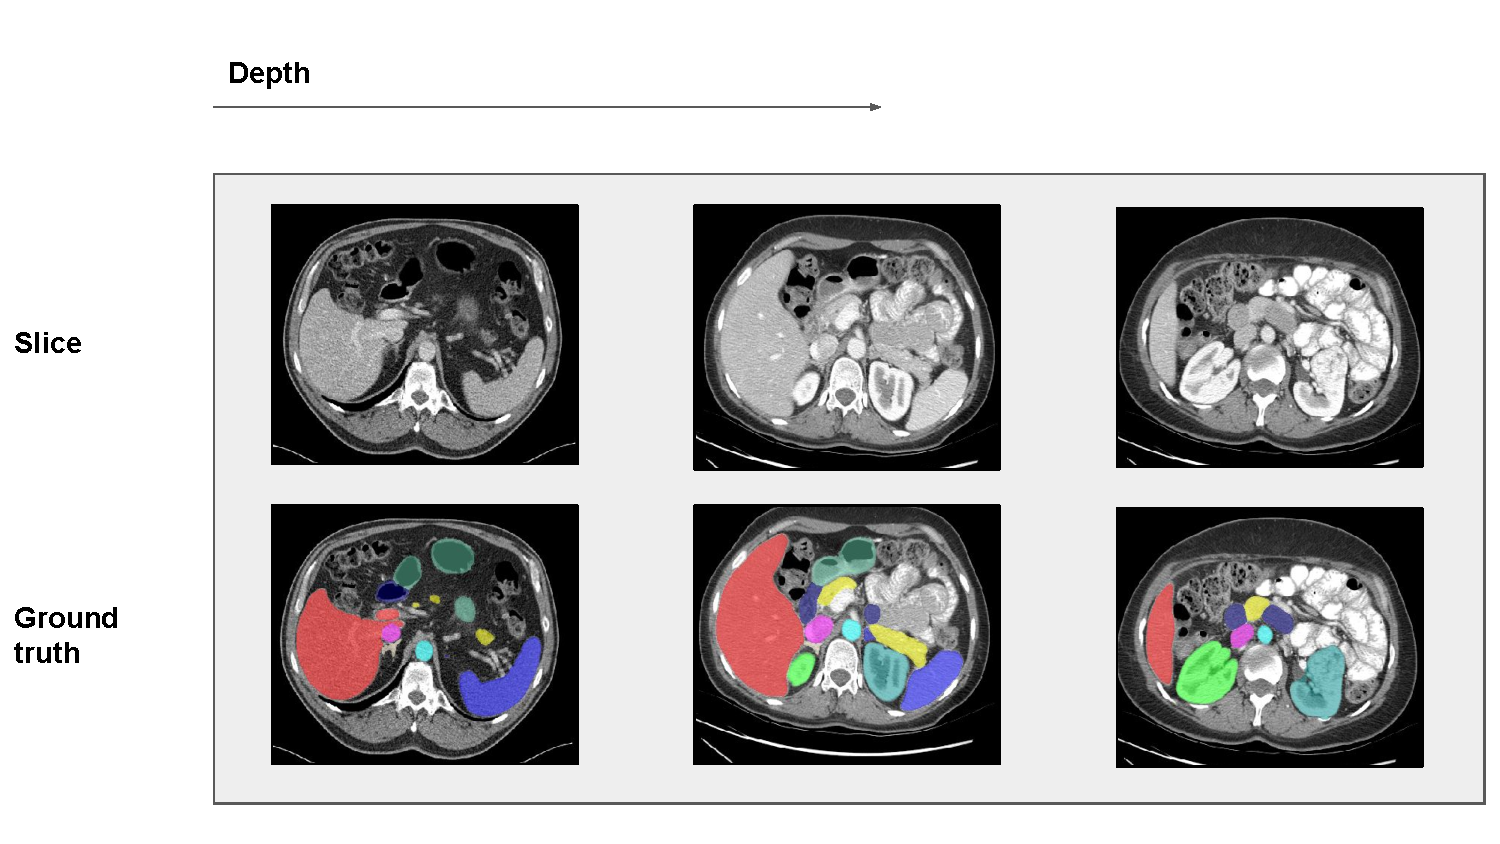
\includegraphics[width=\textwidth]{content/resources/new_images/intro/pipeline.pdf}
    \caption{Slice-level annotation of volume organs segmentation}
    \label{fig:vos}
\end{figure}

In volume object segmentation, there are two main approaches including:
\begin{itemize}
    \item \textbf{Approach by capturing the whole 3D volume:} The state-of-the-art approaches for 3D medical image segmentation are to use a model that has the exact volume and shape of the medical image (figure \ref{fig:vos_3d}). This allows for more 3-dimensional relationships instead of just 2 dimensions, which leads to smoother and more accurate segmentation masks. The model convergence is also faster than techniques that rely on 2d images, and the prediction speed is also satisfactory. However, this approach does have some disadvantages. For example, it highly consumes internal memory resources or needs a complex pre-processing strategy for different configurations like spacing and normalizing. These are sensitive to out-of-distribution data and can lead to terrible predictions. 
    
    \begin{figure}[!h]
        \centering
        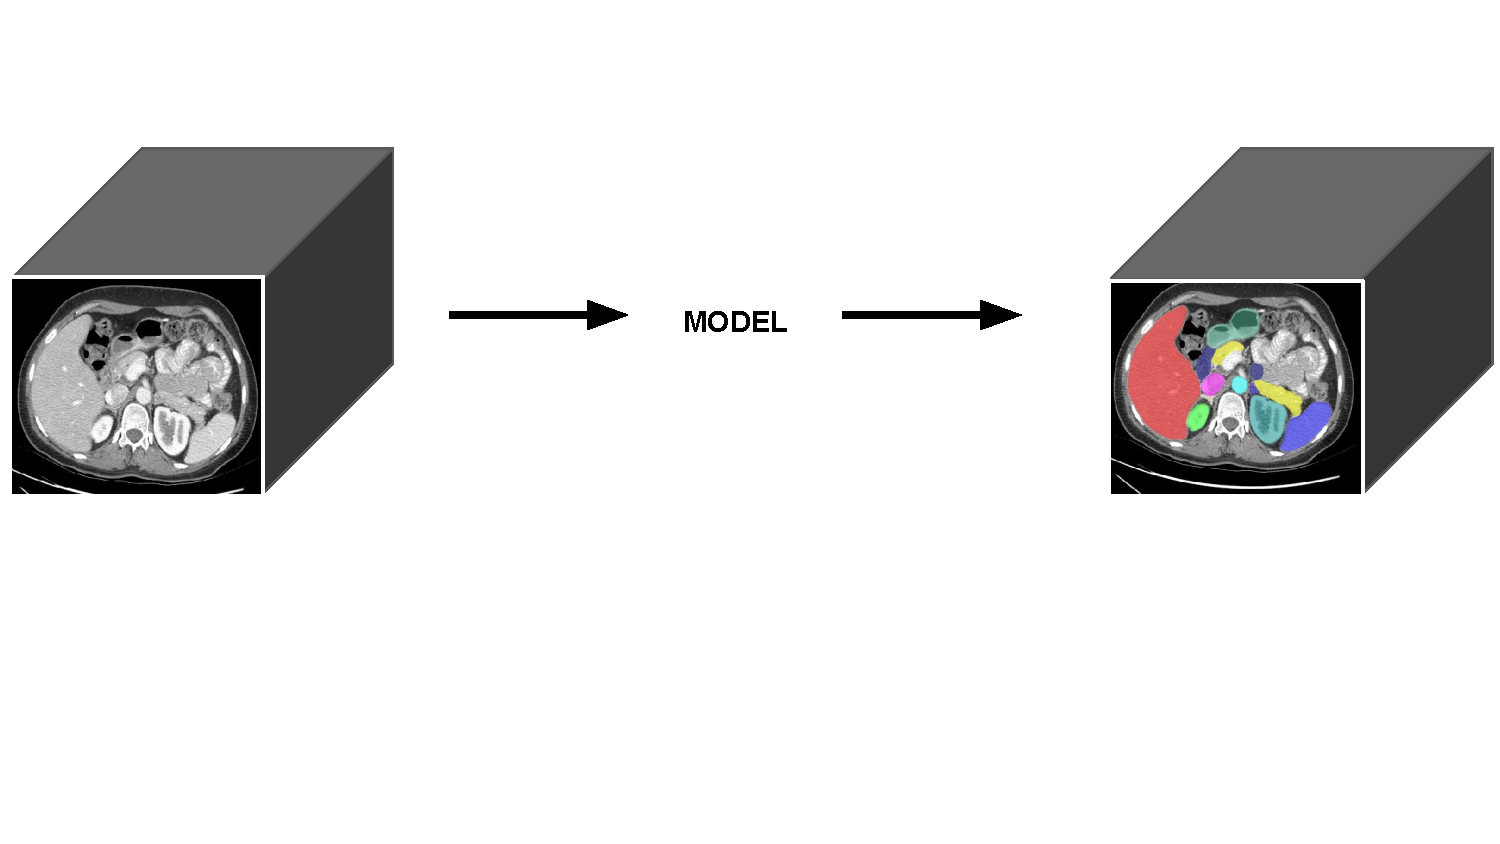
\includegraphics[width=\textwidth]{content/resources/new_images/intro/3d_approach.pdf}
        \caption{The normal pipeline for CT volume object segmentation}
        \label{fig:vos_3d}
    \end{figure}
    
    \item \textbf{Approach by looping slice by slice through the volume (figure \ref{fig:vos_2d}):} for this approach, the analyzing progress is as same as for video sequence data. Since the computational cost is light enough, the image input to the models can keep the original resolution instead of having to be reduced as 3D models usually handle. Furthermore, by looping and keeping temporary memory, the model focuses on just a part of the volume, which makes it avoid redundancy information. The fatal disadvantage of the two-dimensional approaches to medical images is that they are not possible to see the entire object at once like in 3D space. This causes defects in distantly dissected parts, making it difficult for the model to retrieve information from slices that are far apart. Because of that, the development of 2D models in research for medical images is lacking and not many people try to improve the results. However, we think that this approach has a lot of potentials and can be developed into common behaviors based on doctors' habits or knowledge. We aim to make the model transferable between different domains so that it can be used more effectively. But with our targets, the challenges we facing is also daunting. Since we are treating the 3d volume as a video, and because it often requires attentive handling of object interaction, occlusion, distortion, motion blur, scaling, and tracking through the frame, we also have to handle challenges like being out of view, small objects, suddenly appearing, objects disappearing, and reappearing. The model needs to gain time-spatial understanding to prove more beneficial in many ways.
    
    \begin{figure}[!h]
        \centering
        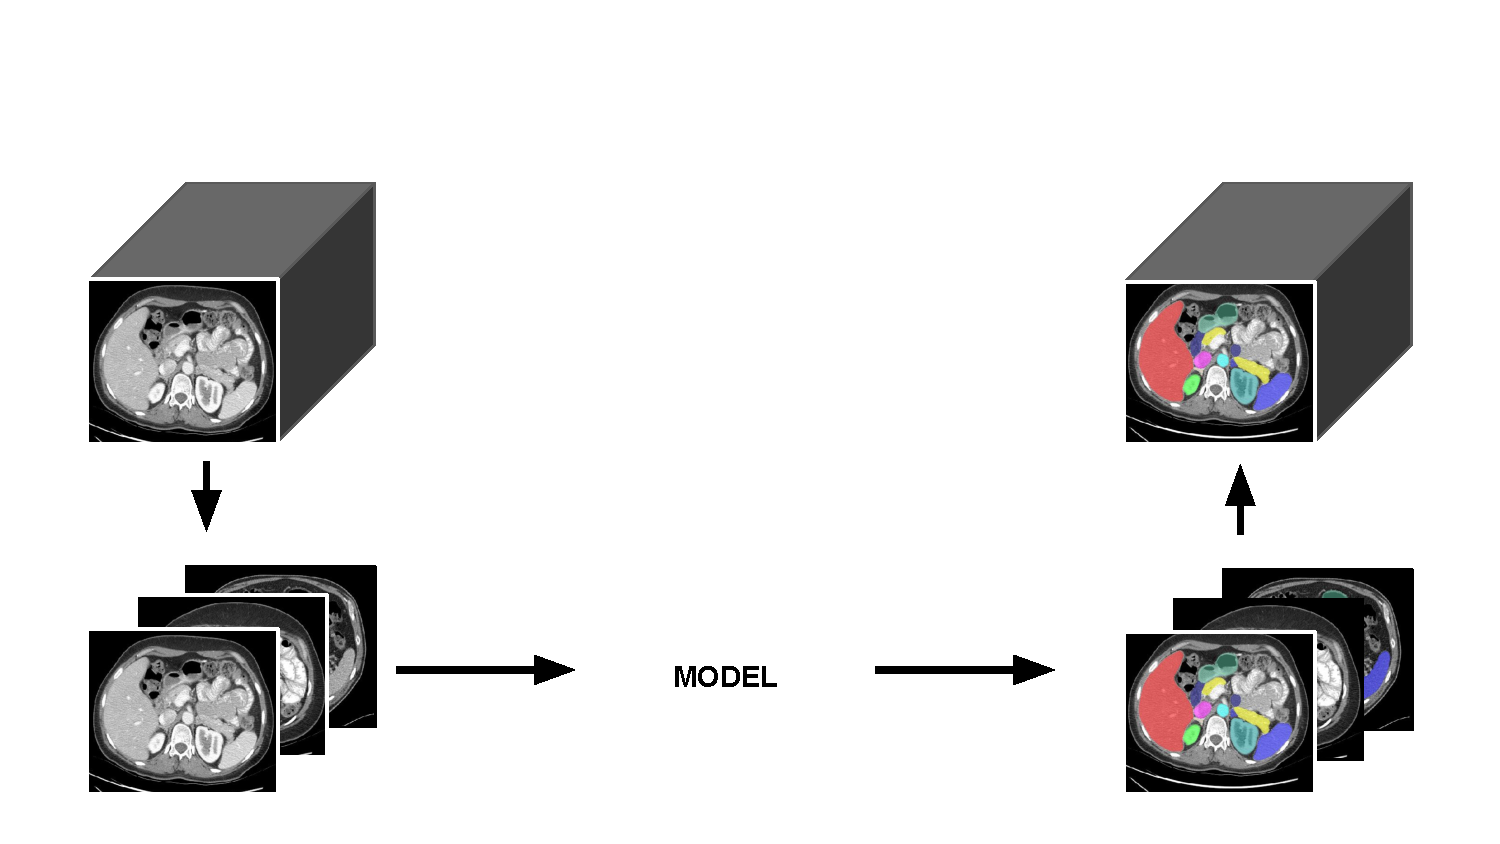
\includegraphics[width=\textwidth]{content/resources/new_images/intro/2d_approach.pdf}
        \caption{2D pipeline approach for CT volume object segmentation}
        \label{fig:vos_2d}
    \end{figure}
    
\end{itemize}


\subsection{Interactive CT Volume Organ Segmentation}
% interactive scenario là gì?
% Là quy trình gán nhãn - refined được lặp đi lặp lại bán tự động hoá (semi automated) giúp quá trình annotate diễn ra nhanh hơn. Thuật toán sẽ dựa theo đối tượng mà người dùng chú ý để interpolate ra các frame còn lại.
% why interactive?
% Như đã đề cập, việc gán nhãn cho các mô hình tốn chi phí khổng lồ, đặc biệt khan hiếm. Nên việc phát triển các thuật toán cho medical bị hạn chế rất nhiều. Xét ngữ cảnh bán tự động hoá, khi mà thuật toán còn chưa hoàn thiện thì việc gán nhãn bán tự động là cần thiết khi nhân lực expert khan hiếm và khó đào tạo, như cầu tạo ra các bộ dữ liệu 3D rất cần thiết. interactive scenario giúp tăng tôc quá trình gán nhãn như human-in-the-loop. Số nhãn không cần biết trước contribute rất nhiều cho nguồn dữ liệu.
% how to interact?
% Người gán nhãn còn được gọi là annotator, 
% Chọn 1 frame valuable nhất và tiến hành vẽ nguệch ngoạc cho từng đối tượng trong khung này. Dựa trên những nét vẽ nguệch ngoạc này, mô hình phải dự đoán segmentation mask của những đối tượng đó. Mô hình sẽ propagate cho tất cả các slices trong volume. Trong tương tác tiếp theo, annotator chọn một slice độ chính xác kém nhất và cung cấp một tập hợp nguệch ngoạc trong khung này. Những nét vẽ nguệch ngoạc này chỉ ra các positive pixel và negative pixels bằng cách đánh dấu các false positive và false negative.
% Quy trình này được lặp lại cho đến khi người chú thích hài lòng với việc phân đoạn mặt nạ của tất cả các khung.
% Expectation:
% Các phương pháp để giải quyết nhiệm vụ phân đoạn đối tượng volume tương tác phải đáp ứng nhiều mục tiêu, bao gồm nhanh chóng, đánh giá định lượng tốt, tạo ra kết quả ban đầu đủ để thoả mãn user và cải thiện độ chính xác cao sau các lần tương tác.
% \lipsum[2]
The process of volume object segmentation is an important tool for analyzing medical images. By labeling and refining the object boundaries interactively, the doctors can get a better understanding of the image data. However, this process can be time-consuming and tedious. A semi-automated process could help to speed things up without sacrificing accuracy. The algorithm would be based on the user's observations to interpolate the remaining frames. This would allow us to quickly obtain a detailed analysis of medical images while still maintaining precision.

As mentioned above, preparing medical ground truth for the supervised algorithm is resource-intensive. That leads to the limitation of algorithms developed for medical diagnosis and treatment. Considering the semi-automated context, when the algorithm is still incomplete, semi-automatic labeling is necessary when expert manpower is scarce and takes years of training. Therefore, 3D dataset creation using interactive scenario appears to tackle this problem and speed up the labeling process as human in a loop. Unlabelled data takes a lot of benefits from this appearance.

The process of interactive volume object segmentation is as follows: the doctor, also known as an annotator, selects the most valuable frame and proceeds to label each object in this frame. Based on this data, the model task is to predict the segmentation mask of those objects in the remaining slices of volume by propagating the annotation throughout it. In the next interaction, the annotator selects a slice with the highest uncertainty and provides suggestions as to the corresponding scribbles in this slice. These scribbles indicate positive pixels and negative pixels by marking false positives and false negatives. This interaction between doctors and models allows for more accurate predictions and helps ensure that results are as accurate as possible. This process is repeated until the annotator is satisfied with the resulting segmentation of the entire volume.

\begin{figure}[h]
    \centering
    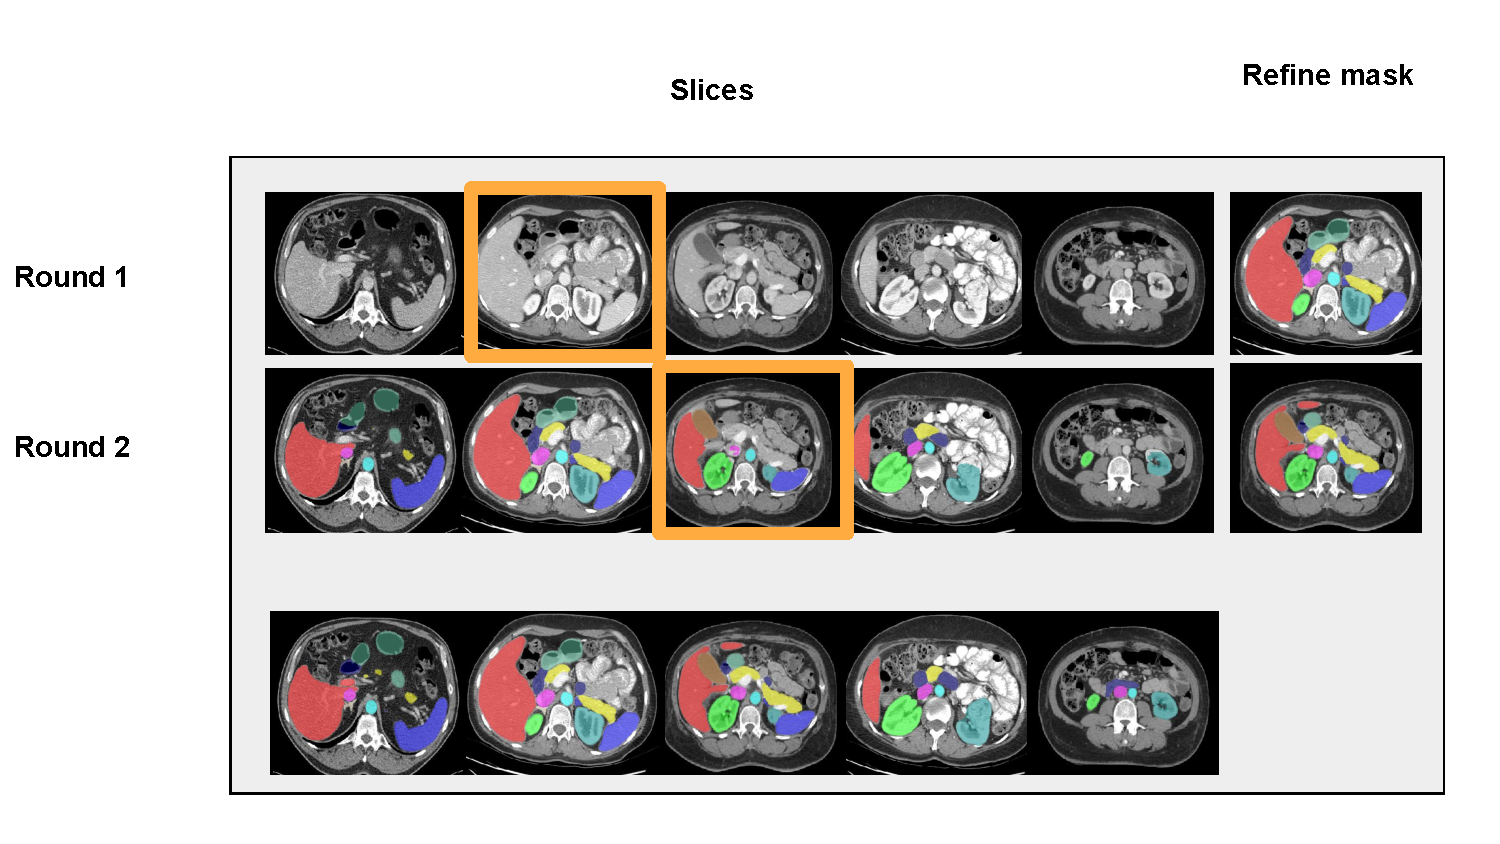
\includegraphics[width=\textwidth]{content/resources/new_images/intro/interactive.pdf}
    \caption{Round-based interactive volume organs segmentation.}
    \label{fig:ivos}
\end{figure}


There are many different ways to approach the interactive volume object segmentation task. However, we believe the most appropriate method must be to appreciate the significance of multiple criteria when making the decision. Speed is important, as we want to produce initial results that satisfy the user. Reasonable quantitative evaluation is also crucial, as it allows us to improve accuracy after annotator interactions.
